\section{Results}
\label{sec:results}
Table~\ref{tab:conditions} shows all four training/input cells, and Table~\ref{tab:main-results} reports the matched-pipeline effects and intervals. On PRDECT-ID, the word SVM gained 0.0076 macro-F1, the character SVM gained 0.0013, and mean IndoBERT fell by 0.0034; all three nominal intervals include zero. On SmSA, the word and character SVM effects were 0.0064 and 0.0103, respectively, with intervals spanning zero. Mean IndoBERT improved by 0.0202, with an interval of [0.0037, 0.0381]. Although this interval is above zero, its lower bound is below the pre-experiment practical threshold of 0.01. Thus none of the six intervals supports a gain exceeding that threshold under the specified rule. Fig.~\ref{fig:effects} displays these estimates and intervals.

\begin{table}[t]
\caption{Held-Out Matched-Pipeline Macro-F1 and Normalization Effects}
\label{tab:main-results}
\centering\small
\setlength{\tabcolsep}{2.8pt}
\begin{tabular}{llrrrl}
\hline
\textbf{Data} & \textbf{Model} & $\boldsymbol{O/O}$ & $\boldsymbol{N/N}$ & $\boldsymbol{\Delta}$ & \textbf{95\% CI} \\
\hline
PRDECT & Word & .9570 & .9646 & +.0076 & [$-.0013$, +.0177] \\
 & Char. & .9595 & .9608 & +.0013 & [$-.0076$, +.0101] \\
 & BERT & .9844 & .9810 & $-.0034$ & [$-.0097$, +.0025] \\
SmSA & Word & .7350 & .7414 & +.0064 & [$-.0135$, +.0297] \\
 & Char. & .7214 & .7317 & +.0103 & [$-.0046$, +.0267] \\
 & BERT & .8830 & .9032 & +.0202 & [+.0037, +.0381] \\
\hline
\end{tabular}
\par\vspace{2pt}
\raggedright\small $O/O$ and $N/N$ denote matched training/evaluation conditions. BERT values are means over three seeds. Intervals are nominal, paired, and conditional on the fitted models.
\end{table}

\begin{figure*}[t]
\centering
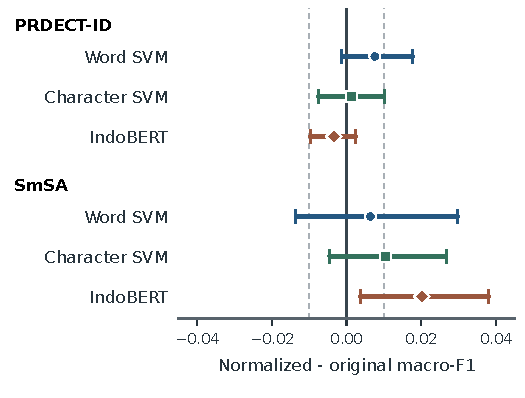
\includegraphics[width=\textwidth]{figures/normalization_effects.pdf}
\caption{Normalized-minus-original pipeline macro-F1 with nominal 95\% paired group-bootstrap percentile intervals. Dashed lines mark the investigator-selected $\pm0.01$ practical margin; seed standard deviations describe variation across three IndoBERT effects separately.}
\label{fig:effects}
\end{figure*}

The paired standard deviations of the three IndoBERT effects were 0.0090 for PRDECT-ID and 0.0088 for SmSA. Supplementary Table S1 lists the paired score and difference for each seed on the same held-out reviews; the seeds do not create independent test samples. These standard deviations describe seed variation, whereas the intervals describe resampling uncertainty conditional on the fitted models. They are not interchangeable, and the nominal intervals are not simultaneous guarantees across the six effects and four contrasts.

\subsection{Direct Representation Contrasts}
Table~\ref{tab:contrasts} reports the four predefined differences between normalization effects. All four intervals include zero. In particular, the apparently larger SmSA IndoBERT effect does not by itself establish that its normalization effect differs from the word SVM's effect. These intervals also do not establish equivalence between representations.

\begin{table}[t]
\caption{Direct Contrasts Between Normalization Effects}
\label{tab:contrasts}
\centering\small
\setlength{\tabcolsep}{4pt}
\begin{tabular}{llrl}
\hline
\textbf{Data} & \textbf{Contrast} & \textbf{Estimate} & \textbf{95\% CI} \\
\hline
PRDECT & Word $-$ character & +.0063 & [$-.0038$, +.0178] \\
 & Word $-$ IndoBERT & +.0110 & [$-.0004$, +.0233] \\
SmSA & Word $-$ character & $-.0039$ & [$-.0303$, +.0226] \\
 & Word $-$ IndoBERT & $-.0138$ & [$-.0384$, +.0105] \\
\hline
\end{tabular}
\par\vspace{2pt}
\raggedright\small Intervals use the same paired group draws as the pipeline effects.
\end{table}

\subsection{Class and Fixed-Model Diagnostics}
Table~\ref{tab:classes} summarizes class F1 with unique-review support; Supplementary Table S2 gives four-decimal values. On SmSA, the word SVM's neutral F1 increased while its negative and positive F1 declined. IndoBERT's mean neutral F1 also increased. These class results are descriptive, not separately adjusted tests.

\begin{table*}[t]
\caption{Held-Out Class F1 for Matched Pipelines}
\label{tab:classes}
\centering\small
\setlength{\tabcolsep}{6pt}
\begin{tabular}{llrrrrrrr}
\hline
\textbf{Data} & \textbf{Class} & \textbf{Support} & \multicolumn{2}{c}{\textbf{Word SVM}} & \multicolumn{2}{c}{\textbf{Character SVM}} & \multicolumn{2}{c}{\textbf{IndoBERT}} \\
 & & & $O/O$ & $N/N$ & $O/O$ & $N/N$ & $O/O$ & $N/N$ \\
\hline
PRDECT & Negative & 412 & .9593 & .9666 & .9618 & .9631 & .9852 & .9820 \\
 & Positive & 381 & .9547 & .9626 & .9572 & .9585 & .9836 & .9801 \\
SmSA & Negative & 204 & .8426 & .8337 & .8145 & .8238 & .9372 & .9495 \\
 & Neutral & 88 & .5263 & .5674 & .5507 & .5612 & .7769 & .8248 \\
 & Positive & 208 & .8363 & .8232 & .7990 & .8103 & .9348 & .9352 \\
\hline
\end{tabular}
\par\vspace{2pt}\small Supports count distinct test reviews; IndoBERT values are means of seed-specific F1, not pooled predictions.
\end{table*}

Table~\ref{tab:transitions} gives both fixed-model input directions. For an original-trained model, the reported change is $O/N-O/O$; for a normalized-trained model, it is $N/O-N/N$. Counts describe transitions from $O/O$ to $O/N$ and from $N/N$ to $N/O$, respectively. IndoBERT entries are means across the three seeds on the same reviews, not unique-review totals; Supplementary Table S3 also reports distinct-review unions.

\begin{table}[t]
\caption{Fixed-Model Macro-F1 Changes and Prediction Transitions}
\label{tab:transitions}
\centering\small
\setlength{\tabcolsep}{2.5pt}
\begin{tabular}{llll}
\hline
\textbf{Data} & \textbf{Model} & $\boldsymbol{O/N-O/O}$ & $\boldsymbol{N/O-N/N}$ \\
\hline
PRDECT & Word & $+.0013$ (10/9) & $-.0277$ (7/29) \\
 & Char. & $+.0051$ (5/1) & $-.0113$ (8/17) \\
 & BERT & $-.0008$ (.67/1.33) & $.0000$ (1.67/1.67) \\
SmSA & Word & $+.0016$ (1/0) & $-.0056$ (1/3) \\
 & Char. & $+.0030$ (2/0) & $+.0025$ (1/1) \\
 & BERT & $+.0006$ (.33/.33) & $+.0023$ (1.33/0) \\
\hline
\end{tabular}
\par\vspace{2pt}\raggedright\small Each entry is macro-F1 change (corrected/introduced errors). BERT counts are seed means, not unique reviews; changes are rounded to four decimals.
\end{table}

For SmSA IndoBERT, the matched-pipeline change was $+.0202$, whereas applying $N$ to the original-trained model changed macro-F1 by $+.0006$ and changed one prediction per seed on average. These are different comparisons. Their difference does not causally separate substitution, retraining, or independently selected hyperparameters.

\section{Discussion and Limitations}
The research questions receive different levels of resolution. For RQ1, all direct-contrast intervals include zero, leaving representation differences unresolved rather than establishing equivalence. For RQ2, point estimates differ descriptively by dataset: the SmSA IndoBERT interval is positive, while the PRDECT-ID IndoBERT interval crosses zero. The PRDECT-ID word interval spans a small negative value through a gain above 0.01, and the SmSA IndoBERT interval spans positive effects both below and above that margin. These ranges leave materially different outcomes unresolved. For RQ3, fixed-model input switches corrected and introduced errors in both directions (Table~\ref{tab:transitions}).

For practice, the relevant decision is to evaluate a complete preprocessing and training configuration on data representative of its intended use. Adding substitution only at inference is a separate decision, because the fixed-model results need not equal a separately tuned pipeline difference. Potential explanations involving feature sharing, subword robustness, or training adaptation are post hoc hypotheses, not mechanisms established by these comparisons. In particular, the observed SmSA IndoBERT pipeline and fixed-model differences do not identify separate causal contributions of substitution, retraining, or tuning.

The findings are limited to two datasets, one dictionary policy, and one pretrained transformer. The dictionary changed 489 of 793 PRDECT-ID test reviews and 97 of 500 SmSA reviews; only 15 changed SmSA reviews were neutral. Matches are not independently verified slang annotations, and sentiment scores do not establish semantic preservation. IndoBERT uses only three seeds; the nominal test-sample intervals are conditional on fitted models and do not provide simultaneous coverage. Pretraining overlap cannot be excluded, and normalization-only runtime was not measured.

The SVM selection was bound to local checkpoint hashes before test inference. The frozen IndoBERT selection recorded versioned checkpoint identifiers but not whole-weight hashes; all 12 cloud files were hashed subsequently and reproduced their saved validation predictions before held-out inference. This supports execution provenance without a pre-freeze cryptographic binding of the transformer weight bytes.

\section{Conclusion}
A fixed dictionary intervention produced small and uncertain pipeline effects in most tested settings. SmSA IndoBERT showed a positive nominal effect, but its interval did not clear the predefined practical-gain threshold, and direct contrasts did not resolve differences between representations. Fixed-model transitions further show that substitutions can both correct and introduce errors. Broader datasets, dictionary policies, and independently measured preprocessing costs are needed before extending these findings beyond the tested configurations.
